\subsection{Tien Phong warehouse}

\subsubsection{Tien Phong Plastic Joint Stock Company}

Tien Phong Plastic Joint Stock Company is a leading producer and distributor of plastic products in Vietnam \cite{vietnam_report_2021}. The company was established in 1975 and has since become one of Vietnam's largest plastic manufacturers, offering a wide range of products, including plastic pipes, fittings, and packaging materials.

\subsubsection{Tien Phong warehouse}

\paragraph{Layout}\mbox{}

Based on the information in the appendix (see {\autoref{fig:premiese}} and \autoref{fig:design}), it appears that there is currently no shelf or rack system in the warehouse. This can make it difficult to locate and retrieve items quickly, which increases order fulfillment times and negatively impacts overall warehouse operations. While a shelf or rack system is not strictly necessary, it can greatly enhance the efficiency and effectiveness of the warehouse. \cite{rack_system_smart_warehouse}

In order to develop a suitable system and design solution in the later chapters, a custom rack system is recommended. An orthographic projection of each location with a rack system suitable for the carton box (size 40x60x40) has been designed.

    \begin{figure}[!ht]
        \centering
        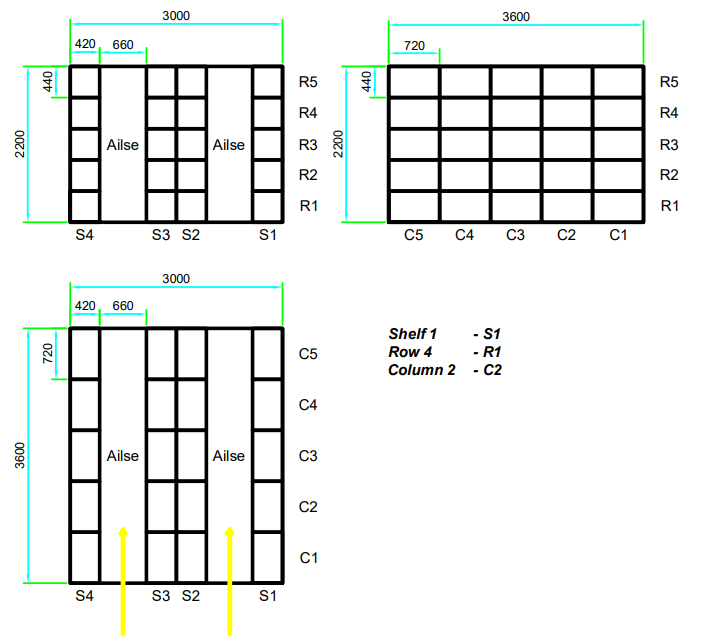
\includegraphics[scale=0.75]{figure/location.png}
        \caption{Orthographic projection of one location}
        \label{fig:location}
    \end{figure}

As shown in \autoref{fig:location}, four shelves with 25 slots each (5x5) have been added. Additionally, there are 2 aisles (0.66 meters) between the shelves at each location.

Based on the recalculations, the storage capacity of each unit is as follows:
\begin{itemize}
    \begin{itemize}
        \item Slot: 0.13 cubic meter;
        \item Shelf: 3.33 cubic meter;
        \item Location: 13.31 cubic meter;
        \item All: 2395.01 cubic meter.
    \end{itemize}
\end{itemize}

It is important to consider orthographic projections of sections in addition to the overall warehouse design. By examining the sections of the warehouse, it is possible to gain a more detailed understanding of how the space can be utilized most effectively.

    \begin{figure}[!ht]
        \centering
        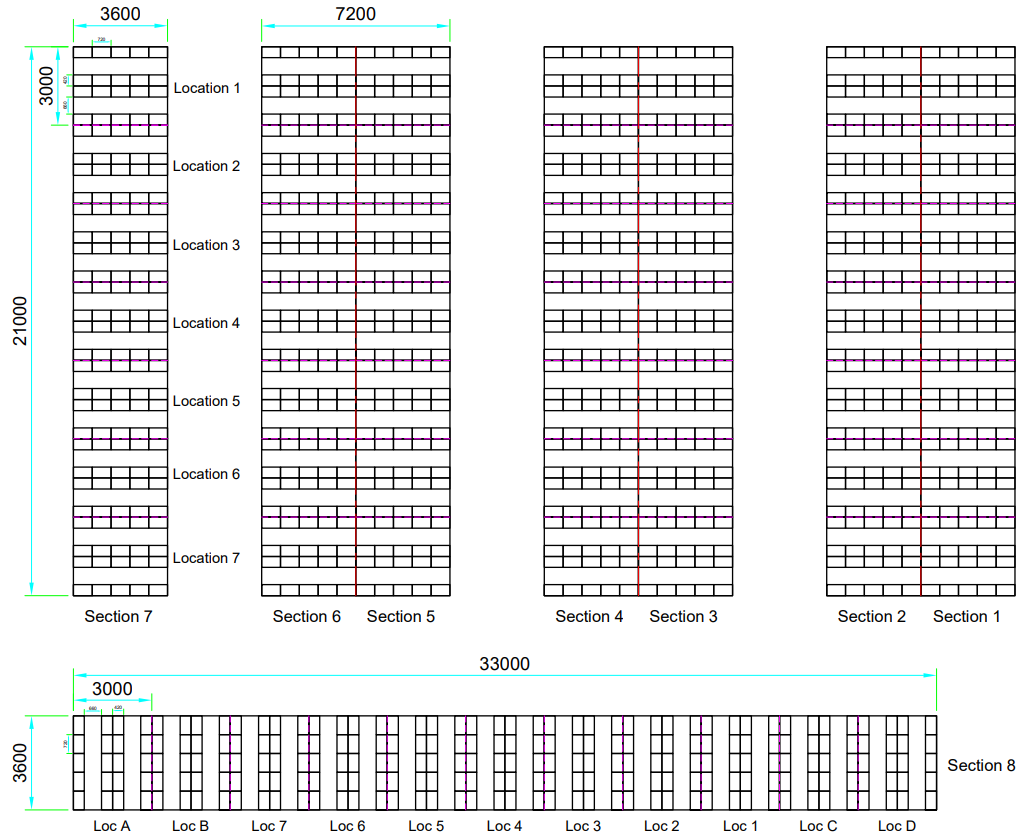
\includegraphics[scale=0.7]{figure/warehouse1.png}
        \caption{Top projection of sections}
        \label{fig:top}
    \end{figure}

In total, TPP's warehouse include: 
\begin{itemize}
    \begin{itemize}
        \item 3 floors;
        \item 8 sections;
        \item 180 locations;
        \item 720 shelfs;
        \item 18000 slots.
    \end{itemize}
\end{itemize}    

    \begin{figure}[!ht]
        \centering
        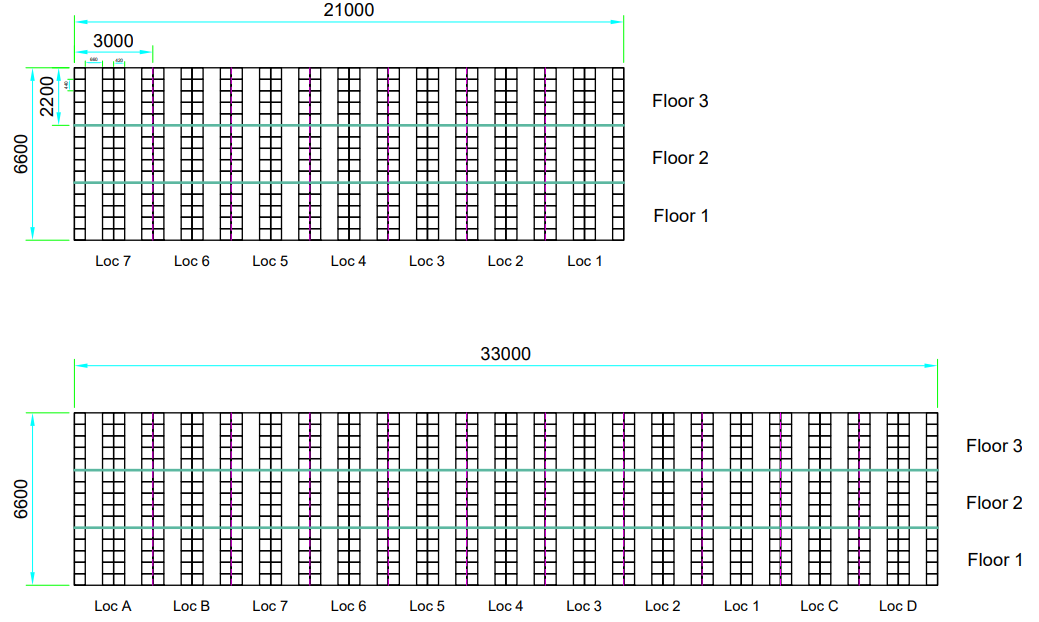
\includegraphics[scale=0.7]{figure/warehouse2.png}
        \caption{Front projection of sections}
        \label{fig:front}
    \end{figure}

    \begin{figure}[!ht]
        \centering
        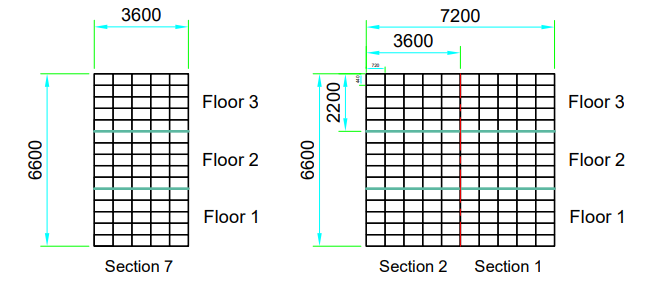
\includegraphics[scale=0.7]{figure/warehouse3.png}
        \caption{Side projections of sections}
        \label{fig:side}
    \end{figure}

\paragraph{Process}\mbox{}

As shown from the report of TPP warehouse (\autoref{fig:manuallabour} and \ref{fig:recinf}), it appears that the current management processes are mostly manual labor, which is both time-consuming and costly. In the span of 10 months, a total of 1,008,832 products (\autoref{fig:rep2019}) were found to be sitting idly in storage in only 4 of the 8 sections. Moreover, the price range of each product varies significantly, from a few thousand to several million Vietnamese dong. The cost of labor and time required to handle such a significant backlog of products is substantial, and it highlights the need for a more efficient and streamlined management process.

Based on analysis of the statistics and research data, It is estimate that with the implementation of the new rack system, each slot will change its contents approximately ten times on average per year. This estimate takes into account factors such as the size and type of items being stored, as well as the expected frequency of inventory turnover. \cite{tienphongplastic}

\subsection{Warehouse management system}

Warehouse management refers to the process of organizing, controlling, and managing the operations of a warehouse. This includes the receipt, storage, and distribution of goods and materials. Warehouse management aims to optimize the use of space, labor, and equipment to ensure that products are stored, tracked, and delivered efficiently. \cite{Kumar2019}

Warehouse management systems (WMS) are software applications that help manage the operations of a warehouse. They provide real-time information about inventory levels, order processing, and shipping. A WMS typically uses technologies such as barcode scanners, RFID tags, and automated material handling equipment to optimize warehouse operations.  \cite{Kumar2019}

The use of a WMS can provide several benefits, including:
\begin{itemize}
    \begin{itemize}
        \item Improved inventory accuracy: A WMS provides real-time information about inventory levels, reducing the risk of overstocking or understocking.
        \item Increased efficiency: By automating warehouse operations, a WMS can reduce the time and labor required to manage inventory, orders, and shipping.
        \item Enhanced customer service: A WMS can help ensure that products are delivered to customers on time and in good condition, improving customer satisfaction.
        \item Cost savings: By optimizing warehouse operations, a WMS can reduce labor costs, minimize inventory holding costs, and reduce shipping expenses.
    \end{itemize}
\end{itemize}

\subsection{Management Process}

\subsubsection{Receiving and put-away}

    \begin{figure}[!ht]
        \centering
        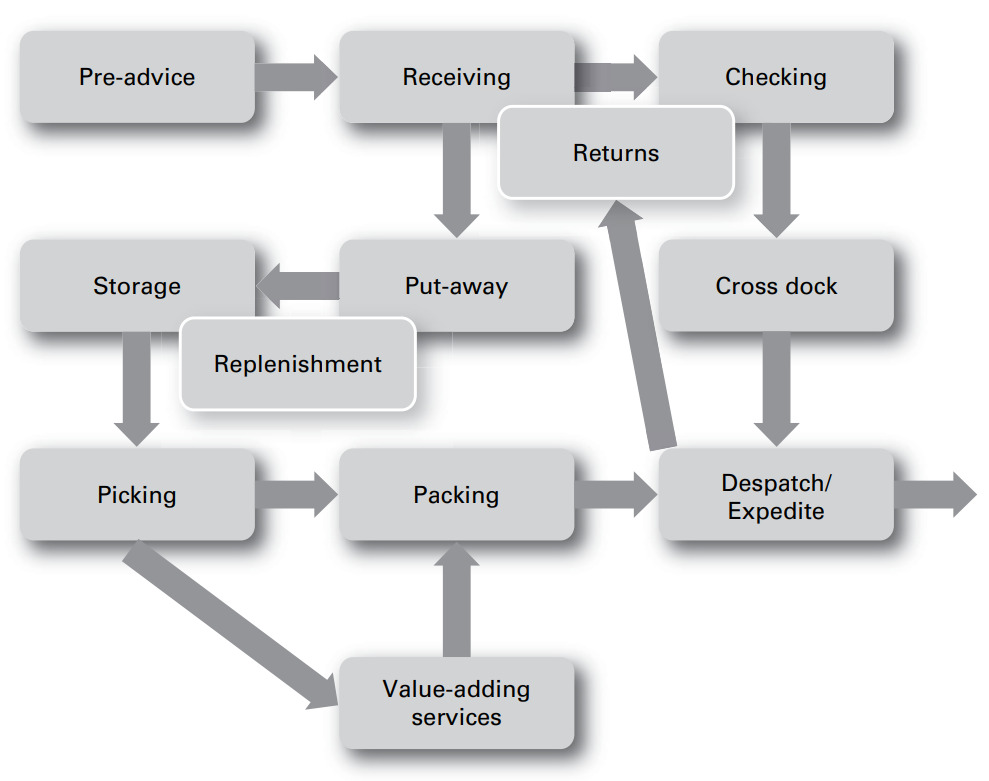
\includegraphics[width=13cm,height=11cm]{figure/processes.png}
        \caption{Receiving and put-away processes}
        \label{fig:wmprocess}
    \end{figure}
    
Although warehouses differ in terms of size, type, function, ownership and location some fundamental processes remain (\autoref{fig:wmprocess}).

\paragraph{Receiving}\mbox{}

Receiving, goods-in or in-handling is a crucial process within the warehouse. 
Ensuring that the correct product has been received in the right quantity and in the right condition at the right time is one of the mainstays of the warehouse operation. These elements are often termed supplier compliance.

\paragraph{In-handling}\mbox{}

One Of the main challenges for a warehouse manager is to match labour hours with work content. Handling a product the least amount of time possible (labour touch points) leads to reduced labour hours and as a consequence, reduced cost. \cite{richards2014warehouse}

Depending on the operation, labour can be the single biggest cost within a warehouse. It can be between 48 and 60 percents Of the total warehouse cost depending on the amount Of automation utilized. It is also the most difficult
cost to control. \cite{richards2014warehouse}

In-handling makes up approximately 20 per cent of the total direct labour
cost within a retail warehouse. \cite{richards2014warehouse}

\paragraph{Put-away}\mbox{}

Many of today's WMSs allocate product locations in advance and instruct the operator as to where to place the goods. This can be directly to the despatch area if the product is to be cross docked as discussed above, to the pick face as a form of replenishment or to a reserve or bulk-storage location.

In order for this system to work effectively, a great deal of information needs to be programmed into the system. This includes the following:
\begin{itemize}
    \begin{itemize}
        \item size, weight and height of palletized goods;
        \item results of an ABC analysis or slotting, where fast-moving goods are
        \item placed closest to the despatch area;
        \item current order data;
        \item family product groups;
        \item actual sales combinations;
        \item current status of pick face for each product.
    \end{itemize}
\end{itemize}

\subsubsection{Order picking}

    \begin{figure}[!ht]
        \centering
        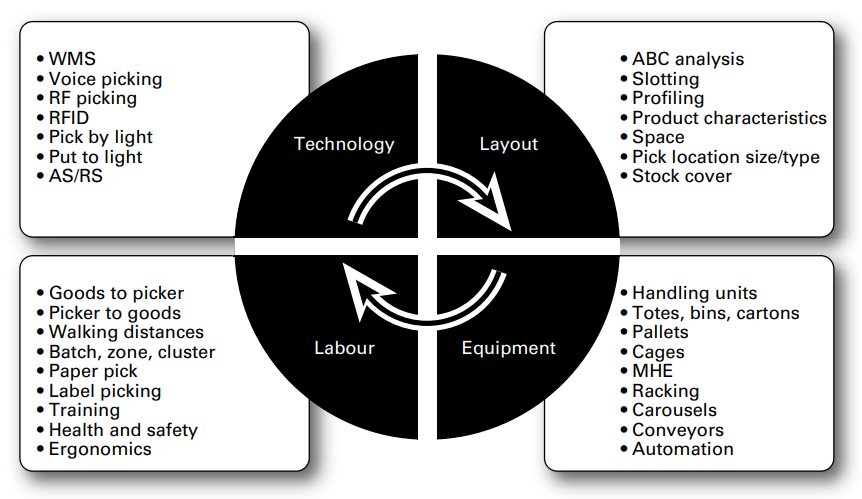
\includegraphics[width=16cm,height=9cm]{figure/picking.png}
        \caption{Picking relationships}
        \label{fig:pickingrelationships}
    \end{figure}

Order picking is the most costly activity within today's warehouses. Not only is it labour intensive, but it is challenging to automate, can be difficult to plan, is prone to error and crucially has a direct impact on customer service (see \autoref{fig:pickingrelationships}). Typical errors include omitting items from the order, sending the wrong item and sending the wrong number of items.

\paragraph{Warehouse pick area layout}\mbox{}

Having produced a comprehensive profile of the products and orders, layout is next to be considered.

    \begin{figure}[!ht]
        \centering
        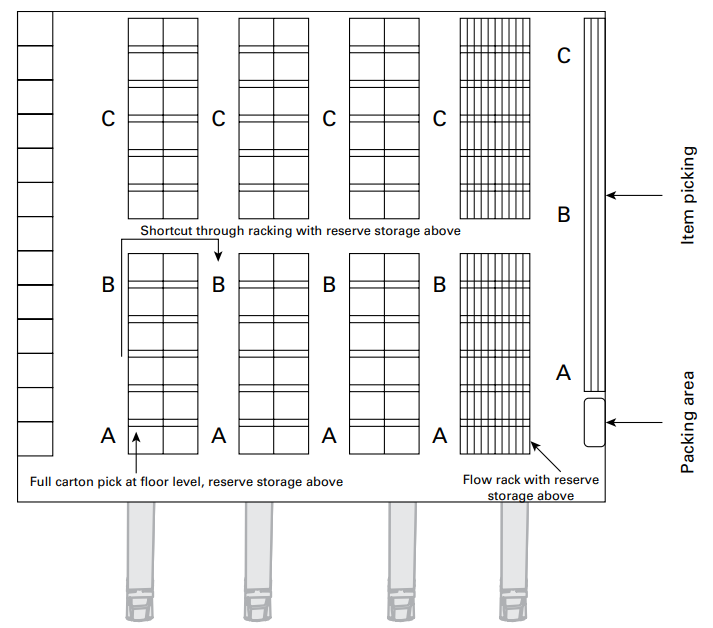
\includegraphics[width=16cm,height=13cm]{figure/layout.png}
        \caption{Sample warehouse layout based on ABC classification}
        \label{fig:layout}
    \end{figure}
    
\autoref{fig:layout} depicts a very basic layout that has used an ABC analysis based on the frequency of pick-face visits. The next step is to minimize the amount of travel through the warehouse when picking an order. \cite{vandenberg2013optimizing}

    \begin{figure}[!ht]
        \centering
        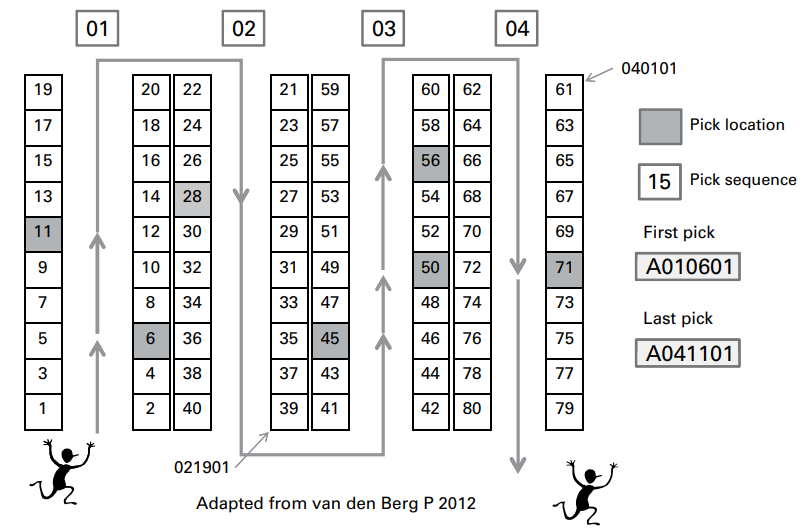
\includegraphics[width=15cm,height=12cm]{figure/sequence.png}
        \caption{Picking route}
        \label{fig:sequence}
    \end{figure} 

The route followed by the picker when assembling the order needs to take into account the following: \cite{vandenberg2013optimizing}
\begin{itemize}
    \begin{itemize}
        \item The pick instruction will have each pick sequenced as per the most effective route beginning at the front of the racking nearest the despatch bays.
        \item Heaviest items are picked first.
        \item The picker should be able to pick from both sides when moving up and down the aisles. See \autoref{fig:sequence} below. In this example the aisles are numbered, not the rows of racking which means that the picker can move from side to side as opposed to travelling up the length of the racking and back down the other side.
        \item Shortcuts are programmed into the system to minimize travel. For example, a break in a long length of racking (as shown in {fig:layout}) enables the picker to shorten the travel distance but allows the storage of reserve product above the pathway.
        \item The picker ends up as close to the despatch area as possible. If the picker is not operating in real time the picker may need to return  to the start point to pick up a new assignment. This is not ideal.
        \item Multiple pick locations for the most popular items need to be set up to avoid congestion at the pick bays.
    \end{itemize}
\end{itemize}

\subsection{Storage strategies}

The organization of warehouses, inputs, and outputs is influenced by what is known as "storage strategies". While these strategies are not primarily focused on what and where items are stored, they do prioritize the structural arrangement of these elements. The most common ones are: FIFO, LIFO, FEFO, HIFO, ...

\subsubsection{FIFO}

FIFO stands for "First-In, First-Out" and is an inventory management method that assumes that the first items received into an inventory are the first to be sold or used. This means that the oldest inventory items are used or sold first, while the newer items are used or sold later. FIFO is commonly used for products that have a limited shelf life or are perishable, such as food or medicine, to ensure that the older items are used first and do not expire. It can also help businesses manage product obsolescence by ensuring that older products are sold or used before newer ones.
   
\subsubsection{LIFO}

LIFO stands for "Last-In, First-Out" and is an inventory management method that assumes that the last items received into an inventory are the first to be sold or used. This means that the newest inventory items are used or sold first, while the older items are used or sold later. LIFO is commonly used for products that have a long shelf life and are not likely to expire or spoil, such as furniture or electronics. It can also help businesses manage rising costs by using the most recently purchased and typically more expensive inventory items first, which can result in lower taxes and higher profits. However, LIFO may not be suitable for businesses that need to track inventory based on expiration dates or other specific characteristics.
    
\subsubsection{FEFO}

FEFO stands for "First-Expired, First-Out" and is an inventory management method that assumes that the first products that will expire are the first to be sold or used. This method is commonly used for products that have a limited shelf life or are perishable, such as food, medicine, or cosmetics. By using the FEFO method, businesses can ensure that they use or sell the products that are closest to their expiration dates first, reducing the risk of spoilage or waste.

\newpage